\documentclass[11pt,a4paper]{article}
\usepackage[a4paper, total={6in, 8in}]{geometry}
\usepackage[latin1]{inputenc}
\usepackage{amsmath}
\usepackage{amsfonts}
\usepackage{amssymb}
\usepackage{graphicx,color}
\usepackage{enumerate}
\usepackage{url}

\title{Simulation experiments for hide-and-seek with different seeker distribution update strategies}
\author{Tirtharaj Dash}
\date{March, 2020}

\begin{document}

\maketitle

\section{Setup}

\noindent
We perform some simulation experiments for Hide-and-Seek with three different \textbf{seeker distribution update strategies}:
\begin{enumerate}[(1)]
	\item\label{snoupd} \textbf{No update:} No update of the seeker distribution (leads to hide-and-seek with replacement results).
	\item\label{supdwor} \textbf{Uniform update:} Open a box, distribute its probability mass to every other unopened boxes, make its probability 0 (hide-and-seek without replacement).
	\item\label{supdhc} \textbf{Hot-cold update:} The seeker updates its probability distribution based on whether it opened a cold box or a hot box. A cold box is a box for which the performance of a box ($perf$) is less than the cold threshold ($\theta_c$) and a hot box is a box with performance greater than a hot threshold ($\theta_h$). We devise the following procedure for update:
	\begin{enumerate}[1.]
		\item Open a box $i$
		\item If $perf(i) \geq \theta_h$: distribute its probability mass to all the unopened boxes in its neighbors. 
		\item If $perf(i) \leq \theta_c$: distribute its probability mass to all the unopened boxes except its neighbors.
		\item If none of 2 or 3: distribute its probability mass to all the unopened boxes.
		\item Repeat 1--4 until the hider is found.
	\end{enumerate}
	\item\label{supdloc} \textbf{Localised-sampling update:} The idea is that if an opened box is a ``good" box then its neighbors may also be good. So, we propose the following update strategy:
	\begin{enumerate}[1.]
		\item Open a box $i$
		\item If the hider is not found in that box, \textbf{but it is a good box (i.e. $perf \geq \theta_h$)}, open its unopened neighbors starightaway and check if the hider is found there.
		\item If hider is not found, then distribute the probability mass of all the boxes (the sampled box and its neighbors) to all unopened boxes equally.
		\item If not 2., then distribute the mass of the opened box $i$ to all unopened boxes equally. 
	\end{enumerate}
\end{enumerate}

\noindent
The seeker update strategy (\ref{supdhc}) requires that the hider distribution falls into some continuity assumption. That is: the probability mass of a neighborhood of a box are in monotonic relationship to the probability of that box. This is a realistic demand and clauses which are related with each other are monotonic in their performance in some fashion. We construct such a hider distribution ($H$) with the following code\footnote{\url{https://github.com/tirtharajdash/multimodalGaussianDistro}}.

\begin{figure}[h]
	\centering
	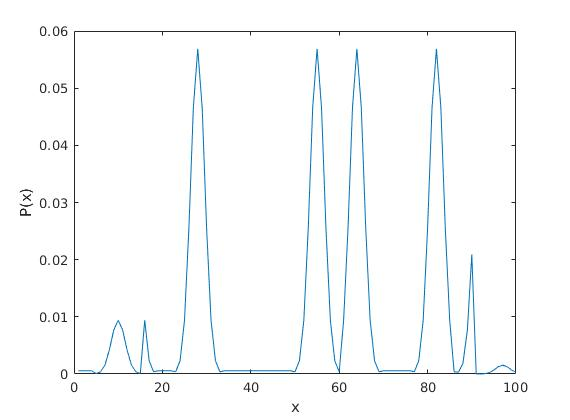
\includegraphics[width=0.5\textwidth]{sample.jpg}
	\caption{Sample hider distibution}
\end{figure}
	

\section{Experiments -- Base} \label{base_expt}

\begin{description}
	\item[Parameter setting] The experiments are performed for number of boxes $n = \{1000, 2000, 3000\}$. The maximum hiding trials is set at $1000$. We call it a \textbf{failure}, if the hider is not found within $n$ searches by using the seeker distribution. The neighborhood size ($nbd$) is varied as \{1,2,3\}. For all the experiments reported here, we define performance of a box by: $perf(i) = \frac{h_i}{\max(h_1,\ldots, h_n)}$, where $H = \{h_1,\ldots, h_n\}$ is the hider distribution. The thresholds are fixed at $\theta_h = 0.80$ and $\theta_c = 0.4$. The proportion of boxes that have high probability mass (spikes in $H$) is fixed at 10\%. For the seeker update stragegy described in \ref{supdloc} requires a neighborhood size ($lnbd$). This is varied as \{1,2,3\}.
	\label{setting:base}

	\item[Results] The mean and standard deviations of misses are calculated only for successful runs i.e. the hider was found by the seeker within maximum of $n$ look-ups. Otherwise, it was treated as a failure and this result was not included for statistics. Below, we report results for each seeker update strategies.
	\begin{figure}[!h]
	\centering
	\begin{tabular}{llll}
		\hline \hline 
		choiceUpdS & SuccessRate & mean(misses) & sd(misses) \\
		\hline \hline 
		\multicolumn{4}{c}{$n = 1000$} \\ 
		\hline 
		1 &  0.622 & 439.738 & 279.218 \\
		2 &  1.000 & 499.379 & 279.060 \\
		3 ($nbd=1$) & 1.000 & 486.041 & 271.251 \\
		3 ($nbd=2$) & 1.000 & 458.027 & 269.987 \\
		3 ($nbd=3$) & 1.000 & 479.270 & 279.110 \\
		4 ($lnbd=1$) & 1.000 & 521.648 & 281.406 \\
		4 ($lnbd=2$) & 1.000 & 559.455 & 283.613 \\
		4 ($lnbd=3$) & 1.000 & 569.803 & 290.259 \\
		\hline 
		\hline 
		\multicolumn{4}{c}{$n = 2000$} \\ 
		\hline 
		1 &  0.635 & 859.123 & 571.302 \\
		2 &  1.000 & 1022.204 & 595.486 \\
		3 ($nbd=1$) & 1.000 & 963.457 & 550.133 \\
		3 ($nbd=2$) & 1.000 & 961.946 & 551.028 \\
		3 ($nbd=3$) & 1.000 & 968.335 & 564.515 \\
		4 ($lnbd=1$) & 1.000 & 1053.850 & 578.713 \\
		4 ($lnbd=2$) & 1.000 & 1118.901 & 560.618 \\
		4 ($lnbd=3$) & 1.000 & 1105.028 & 559.592 \\
		\hline 
		\hline 
		\multicolumn{4}{c}{$n = 3000$} \\ 
		\hline 
		1 &  0.652 & 1303.462 & 854.176 \\
		2 &  1.000 & 1473.717 & 865.756 \\
		3 ($nbd=1$) & 1.000 & 1436.214 & 801.100 \\
		3 ($nbd=2$) & 1.000 & 1396.195 & 840.066 \\
		3 ($nbd=3$) & 1.000 & 1464.990 & 840.695 \\
		4 ($lnbd=1$) & 1.000 & 1611.752 & 872.266 \\
		4 ($lnbd=2$) & 1.000 & 1632.951 & 855.368 \\
		4 ($lnbd=3$) & 1.000 & 1725.939 & 853.418 \\
		\hline 
		\hline 
	\end{tabular}
	\caption{Average number of misses: $H$ is a multimodal distribution with 10\% spikes, and $S$ is updated using three different update strategies (1: no update, 2: without replacement, 3: update using $\theta_h$ and $\theta_c$ using three different neighborhoods in \{1,2,3\}, 4: local sampling based update with local neighborhood in \{1,2,3\}).}
	\end{figure}
		
	\item[Interpretation 1] The results suggest that the threshold based seeker update strategy (\ref{supdhc}):
	\begin{itemize}
		\item Reduces the average number of misses in comparison with search without replacement for which the expected number of misses is $\frac{n-1}{2}$ (i.e. choiceUpdS$=2$ in tables).
		\item For the seeker updat type (\ref{supdhc}), best neighborhood size is found to be 2. 
		\item Increasing the neighborhood size of a box increases the average number of misses in almost all the cases.
	\end{itemize}

	\item[Interpretation 2] The localised sampling based seeker update strategy described in \ref{supdloc} has following effects on average number of misses.
	\begin{itemize}
		\item It is worse than to seeker update strategy \ref{supdhc}.
		\item Bigger neighborhood sizes have adverse effect on the avergae number of misses. This could be due to the fact that we are starting with a uniform neighborhood and we don't have much idea about the true hider distribution yet.
	\end{itemize}
\end{description}

\subsection{Experiments -- Resource-bounded Localised-sampling Update}

The localised sampling update strategy described in \ref{supdloc} contributes a lot of costs towards opening neighbors of a box when the box is a good box. Why does this happen? In the present case, as soon as the seeker finds a good box, it becomes greedy and opens its neighbors. This happens everytime it finds a good box. Opening the neighbors incurs costs, which gets added to the total number of misses. Now, we can restrict this number of neighbor opening to some $MAX\_LS \in (0,1)$ (maximum local sampling), where $MAX\_LS$ could be a function of $n$. We define this constant as follows:
\begin{equation}
MAX\_LS = k*n
\end{equation}
That is neighbor opening is allowed $k$ percentage of $n$ times. We call this strategy as `Resource-bounded localised sampling update'.

\vspace{0.5cm}

\noindent
\textbf{Observation:} It is easy to verify that this is a \textbf{more general} case 
of the seeker update strategy \ref{supdhc} and a \textbf{more specific} case of seeker update strategy \ref{supdloc}. That is:
\begin{itemize}
	\item $MAX\_LS = 0$ results in hot-cold update in \ref{supdhc}.
	\item $MAX\_LS = \infty$ results in localised-sampling update in \ref{supdloc}.
\end{itemize}

\begin{description}
	\item[Results] We conduct experiments with $k = \{0.01, 0.05,0.10\}$. The comparison is against the results obtained for the localised-sampling seeker update (\ref{supdloc}). The neighborhood of a box is fixed at 1. Refer Fig.\ref{fig:resboundedls}.
	\begin{figure}[!h]
		\centering
		\begin{tabular}{llll}
			\hline \hline 
			choiceUpdS & SuccessRate & mean(misses) & sd(misses) \\
			\hline \hline 
			\multicolumn{4}{c}{$n = 1000$} \\ 
			\hline 
			3 ($nbd=1, \textcolor{red}{k = 0}$) & 1.000 & 486.041 & 271.251 \\
			4 ($lnbd=1, \textcolor{red}{k = \infty}$) & 1.000 & 521.648 & 281.406 \\
			4 ($lnbd=1, k = 0.01$) & 1.000 & 512.810 & 283.890 \\
			4 ($lnbd=1, k = 0.05$) & 1.000 & 528.908 & 290.191 \\
			4 ($lnbd=1, k = 0.10$), & 1.000 & 521.648 & 281.406 \\
			\hline 
			\hline 
			\multicolumn{4}{c}{$n = 2000$} \\ 
			\hline 
			3 ($nbd=1, \textcolor{red}{k = 0}$) & 1.000 & 963.457 & 550.133 \\
			4 ($lnbd=1, \textcolor{red}{k = \infty}$) & 1.000 & 1053.850 & 578.713 \\
			4 ($lnbd=1, k = 0.01$) & 1.000 & 986.059 & 573.569 \\
			4 ($lnbd=1, k = 0.05$) & 1.000 & 1031.794 & 572.295 \\
			4 ($lnbd=1, k = 0.10$), &  1.000 & 1053.850 & 578.713 \\
			\hline 
			\hline 
			\multicolumn{4}{c}{$n = 3000$} \\ 
			\hline 
			3 ($nbd=1, \textcolor{red}{k = 0}$) & 1.000 & 1436.214 & 801.100 \\
			4 ($lnbd=1, \textcolor{red}{k = \infty}$) & 1.000 & 1611.752 & 872.266 \\
			4 ($lnbd=1, k = 0.01$) & 1.000 & 1594.132 & 842.846 \\
			4 ($lnbd=1, k = 0.05$) & 1.000 & 1560.329 & 858.586 \\
			4 ($lnbd=1, k = 0.10$), & 1.000 & 1611.752 & 872.266 \\
			\hline 
			\hline 
		\end{tabular}
		\caption{Resource-bounded localised-sampling seeker update.}
		\label{fig:resboundedls}
	\end{figure}

	\item[Interpretation] Here are the observations.
	\begin{itemize}
		\item As $k$ increases, the cost increases. This is expected.
		\item In all cases, $k = 0.10$ results in \ref{supdloc}.
		\item The results are worse than that of the hot-cold update strategy.
	\end{itemize}
	
\end{description}

\section{Conclusions}

The seeker update strategy as described in \ref{supdhc} is the \textbf{best} update strategy, when the hider is not known, but a structural relationship among the boxes is known. The performance 
associated with a box can only be known after opening the box. This kind of hider structure space is applicable to ILP hypothesis space, where the space forms a lattice of clauses and each clause is associated with a performance (e.g. Laplacian smoothed accuracy: $\frac{P+1}{P+N+2}$, where $P$ and $N$ are the number of positive and negative instances respectively).

Our next set of experiments will be testing the applicability of this new seeker update strategy for ILP hypothesis obtained for real-world problems as described in a separate report.

	
\end{document}
